\problema{Agrupamentos}{Leandro Luque (Fatec Mogi das Cruzes)}

Você está trabalhando num projeto que envolve a exibição em um mapa da localização de prestadores de serviço de uma grande empresa. Entre os desafios do projeto está uma lentidão cada vez maior no carregamento do mapa, dado o grande volume de prestadores exibidos - que hoje passa dos 50 mil. Ainda, a visualização do mapa está muito poluída, pois muitos pontos são exibidos em uma área pequena.

Você fez uma PoC (prova de conceito) com uma biblioteca de agrupamento (\textit{clusterização} - que agrupa pontos próximos) do componente de mapas \textit{frontend} que usa e percebeu que o problema de visualização é resolvido. No entanto, agrupar no \textit{frontend} não resolve o problema de ter que carregar milhares de pontos a partir do \textit{backend}. Portanto, você decidiu implementar um algoritmo de clusterização no \textit{backend}. O algoritmo é uma variante do implementado em diversas bibliotecas de mapas disponíveis no mercado.

Em resumo, o algoritmo consiste nos seguintes passos:
\begin{enumerate}
\item Selecione um ponto (no nosso caso, selecionaremos o primeiro ponto na entrada);
\item Verifique qual é o \textit{cluster} mais próximo:
    \begin{itemize}
        \item Se não existir \textit{cluster} mais próximo ou se o \textit{cluster} mais próximo estiver a mais de $x$ unidades de distância (considerando a distância euclidiana entre o ponto e o centro do \textit{cluster}), crie um novo \textit{cluster} com o ponto como seu centro;
        \item Caso contrário, adicione o ponto ao \textit{cluster} mais próximo e recalcule o centro do \textit{cluster} para ser igual a média aritmética das posições de seus pontos constituintes. Caso um ponto esteja à mesma distância de dois ou mais \textit{clusters}, ele deverá ser adicionado ao \textit{cluster} criado primeiro.
    \end{itemize}
\item Selecione o próximo ponto e repita (2) até passar por todos os pontos.
\end{enumerate}

Considere um mapa com os seguintes pontos:
A (7, 7), B (11, 7), C (9, 7), D (6, 8), E (13, 8) - Figura \ref{fig:a}a; e raio do \textit{cluster} igual a 2.

\begin{figure} \centering
    \begin{subfigure}[]{}
        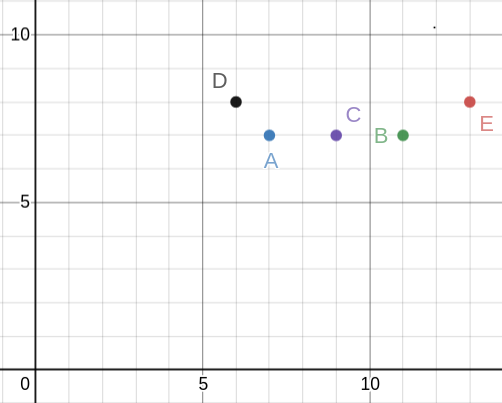
\includegraphics[width=.45\textwidth]{agrupamentos/agrupamentos_1.png}
        \label{fig:a}
    \end{subfigure}\hfill
    \begin{subfigure}[]{}
        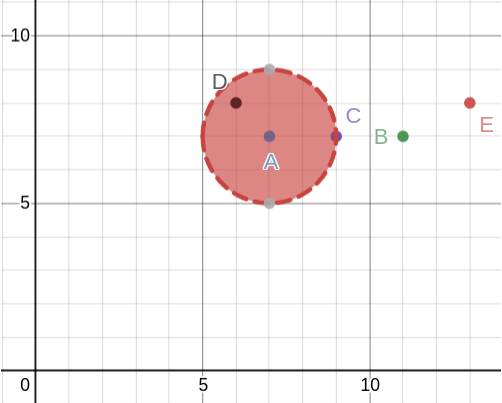
\includegraphics[width=.45\textwidth]{agrupamentos/agrupamentos_2.png}
        \label{fig:b}    
    \end{subfigure}\hfill
    \newline
    
     \begin{subfigure}[]{}
        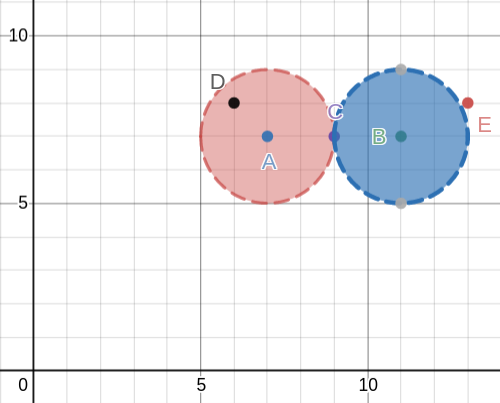
\includegraphics[width=.45\textwidth]{agrupamentos/agrupamentos_3.png}
        \label{fig:c}
    \end{subfigure}\hfill
    \begin{subfigure}[]{}
        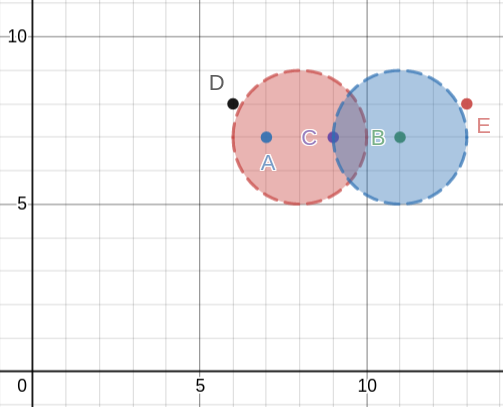
\includegraphics[width=.45\textwidth]{agrupamentos/agrupamentos_4.png}
        \label{fig:d}    
    \end{subfigure}\hfill
    \newline
    
     \begin{subfigure}[]{}
        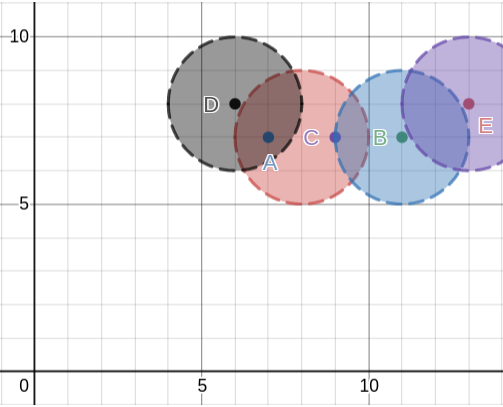
\includegraphics[width=.45\textwidth]{agrupamentos/agrupamentos_5.png}
        \label{fig:e}
    \end{subfigure}\hfill

    \caption{Passo a passo do algoritmo}
\end{figure}

\begin{enumerate}
    \item Começaremos pelo primeiro ponto informado: A (7,7);
    \item Como ainda não existem \textit{clusters}, será criado um novo com centro em (7, 7) - Figura \ref{fig:b}b;
    \item O próximo ponto (B) está à quatro unidades de distância do primeiro \textit{cluster} e, portanto, será criado um novo \textit{cluster} com (11, 7) como centro - Figura \ref{fig:b}c;
    \item O terceiro ponto (C) está a duas unidades de distância do primeiro e do segundo \textit{clusters}. Como as distâncias são iguais, deve-se inclui-lo no primeiro cluster criado (A). Após adicioná-lo, o novo centro do \textit{cluster} deverá ser atualizado para ((xa + xc) / 2, (ya + yc) / 2) = ((7 + 9) / 2, (7 + 7) / 2) = (8, 7) - Figura \ref{fig:b}d;
    \item O mesmo processo segue até o fim, resultando em 4 clusters - Figura \ref{fig:b}e.
\end{enumerate}

Seu trabalho é implementar o algoritmo explicado.

\section*{Entrada}

A entrada começa com uma linha com dois inteiros: $N$ ($1 \leqslant N \leqslant 100$) indicando o número de prestadores de serviço e $R$ ($1 \leqslant R \leqslant 100$) representando o raio que será usado para os \textit{clusters}. As próximas $N$ linhas contêm coordenadas cartesianas $X$ $Y$ inteiras ($-1000 \leqslant X, Y \leqslant 1000$) representando a localização de um prestador de serviço. A última linha de entrada termina com uma quebra de linha.

\section*{Saída}

Como saída, imprima uma linha com um número $C$ indicando o número de \textit{clusters} criados pelo algoritmo. Em seguida, imprima $C$ linhas, cada uma com coordenadas cartesianas inteiras (trucando o resultado se necessário) $X$ $Y$ indicando o centro de cada \textit{cluster}, na ordem em que foram criados. A última linha de saída termina com uma quebra de linha.